\section{Manual Penggunaan Aplikasi}

\subsection{Fitur Tembang}
Dalam Aplikasi ini ada fitur penjelasan tembang dimana user dapat melihat penjelasan tembang tembang bali yang ada.
\subsubsection{Download Aplikasi}
Download Aplikasi dari playstore atau dari \href{https://github.com/rahdeva/tembang_bali}{release repository github berikut.} 

\subsubsection{Install dan Buka Aplikasi}
Install aplikasi dengan klik aplikasi dan menunggu hingga aplikasi terinstall. Dan buka aplikasi dan muncul greeting page.

\begin{figure}[H]
    \centering
    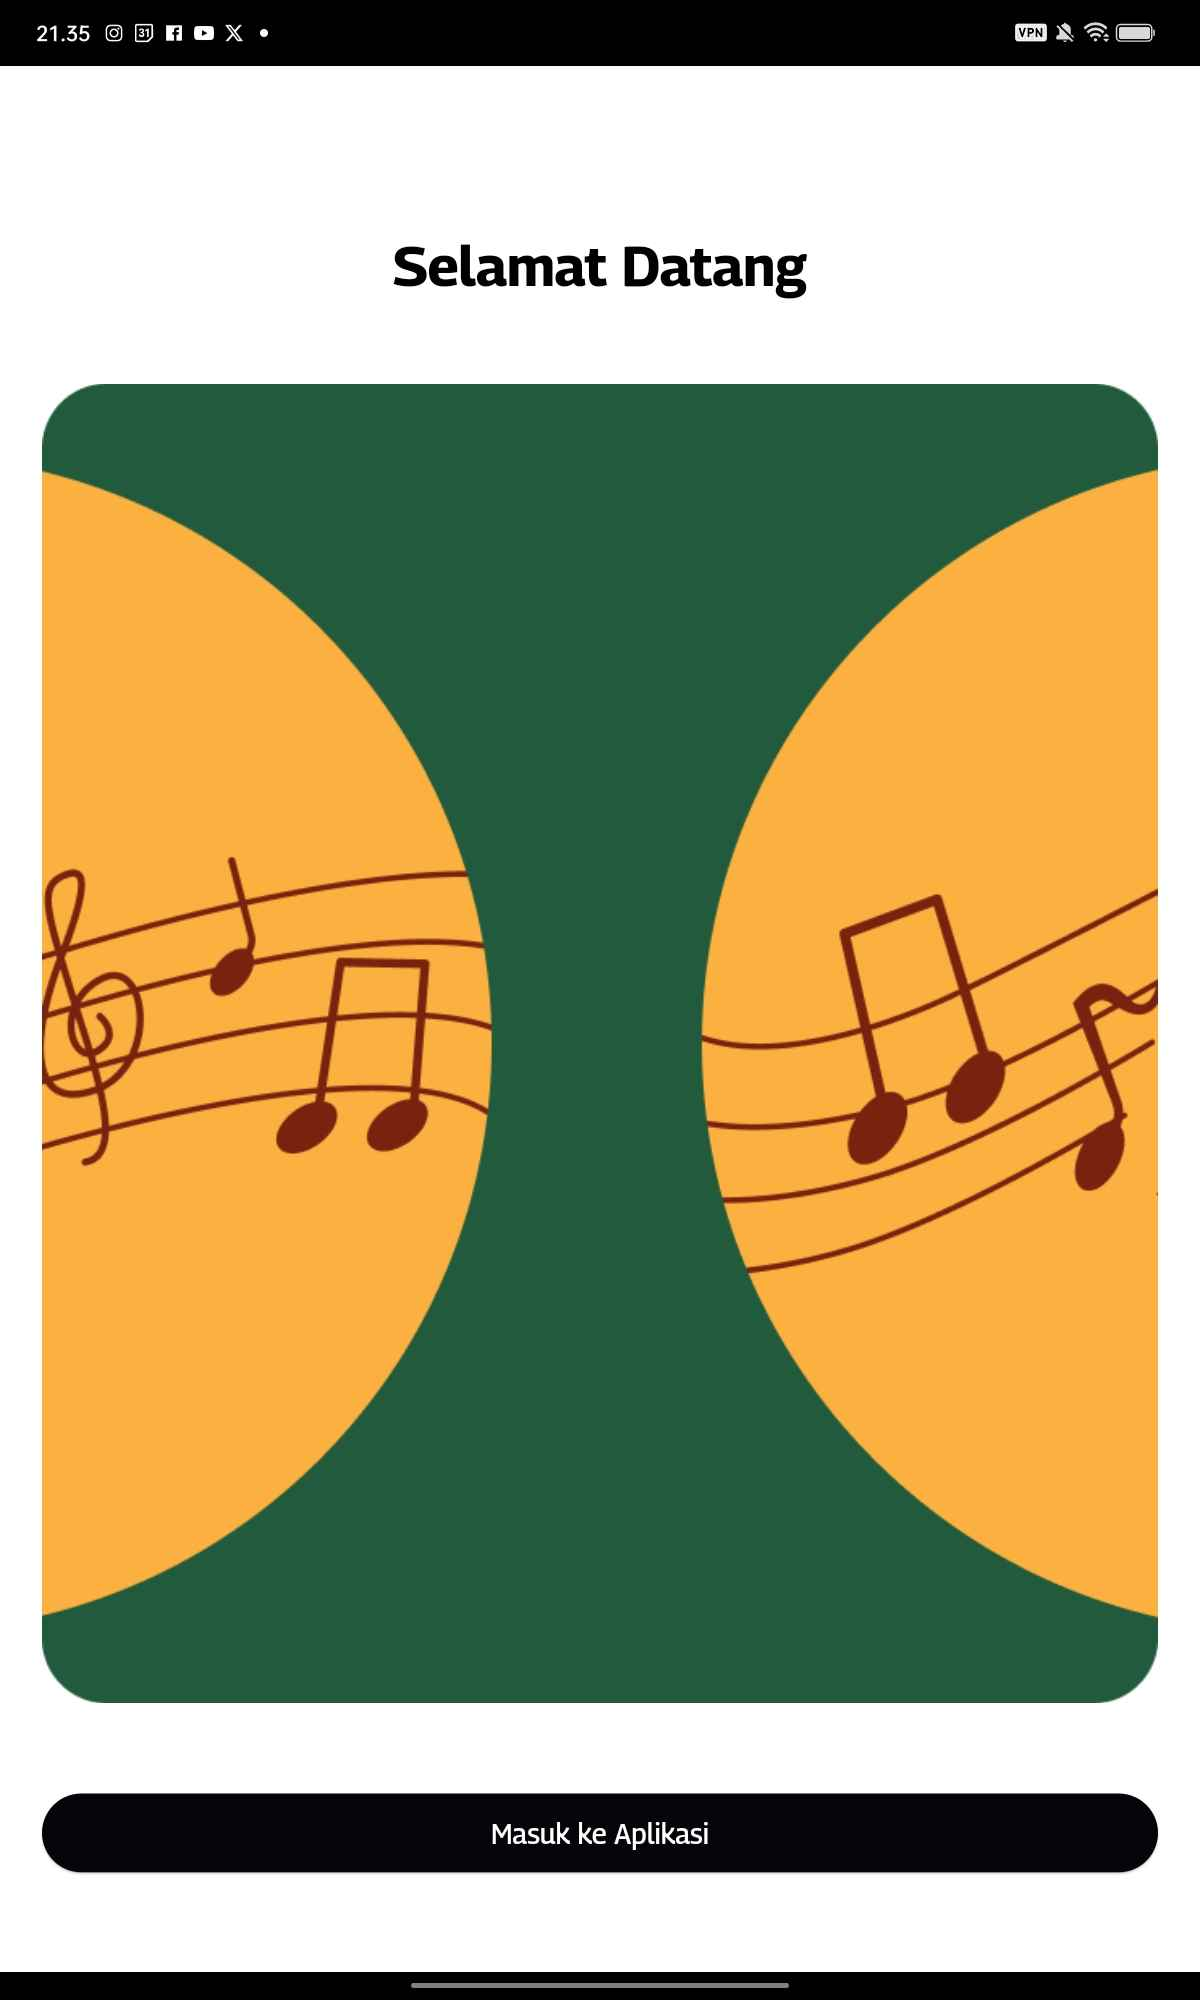
\includegraphics[width=0.3\textwidth]{assets/welcome.jpg}
    \caption{Welcome Page}
\end{figure}

\subsubsection{Pilih Kategori}
Pilih kategori tembang yang diinginkan.

\begin{figure}[H]
    \centering
    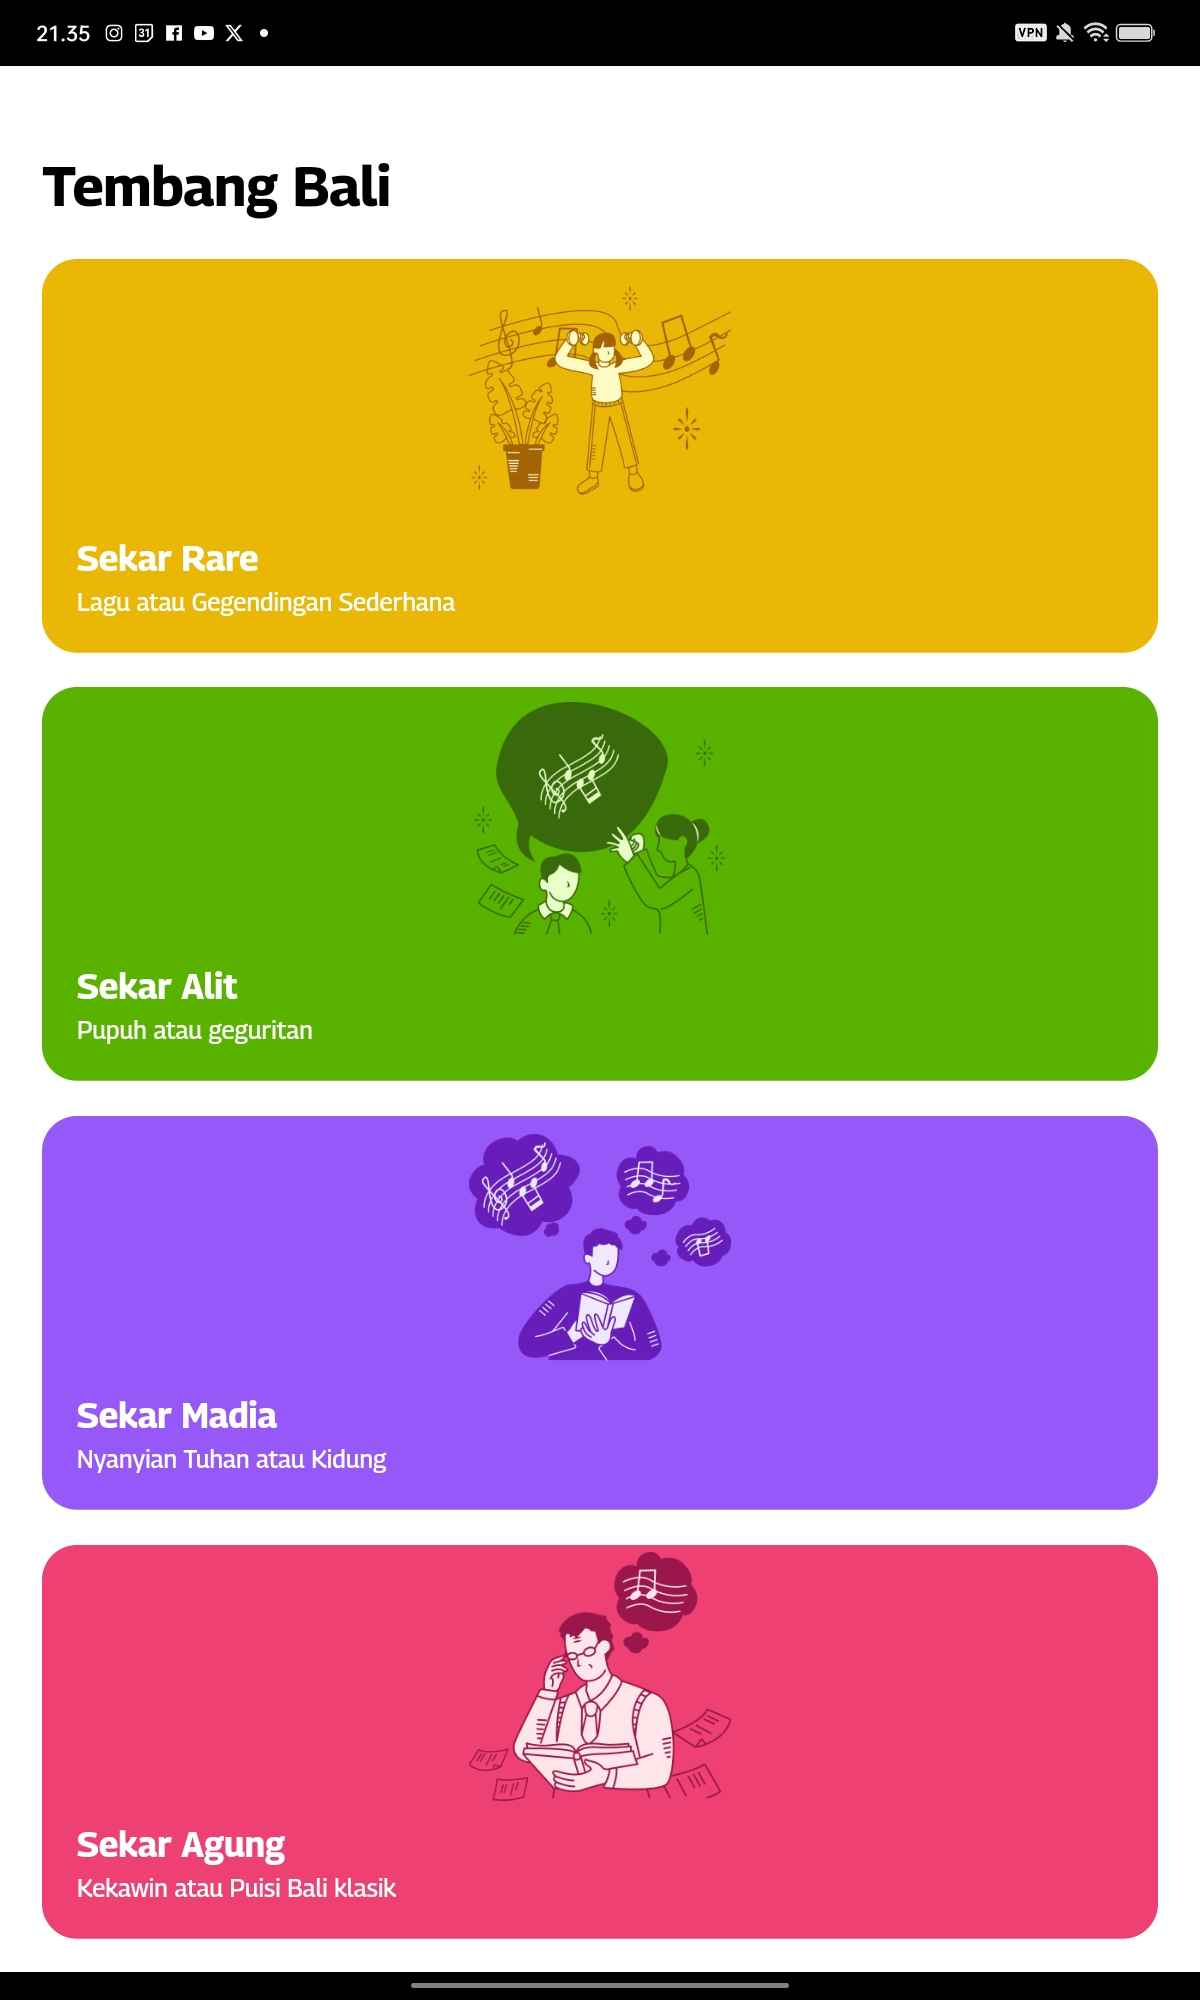
\includegraphics[width=0.3\textwidth]{assets/list-gita.jpg}
    \caption{List Dharma Gita}
\end{figure}

\subsubsection{Pilih Tembang}
Pilih salah satu tembang yang diinginkan.

\begin{figure}[H]
    \centering
    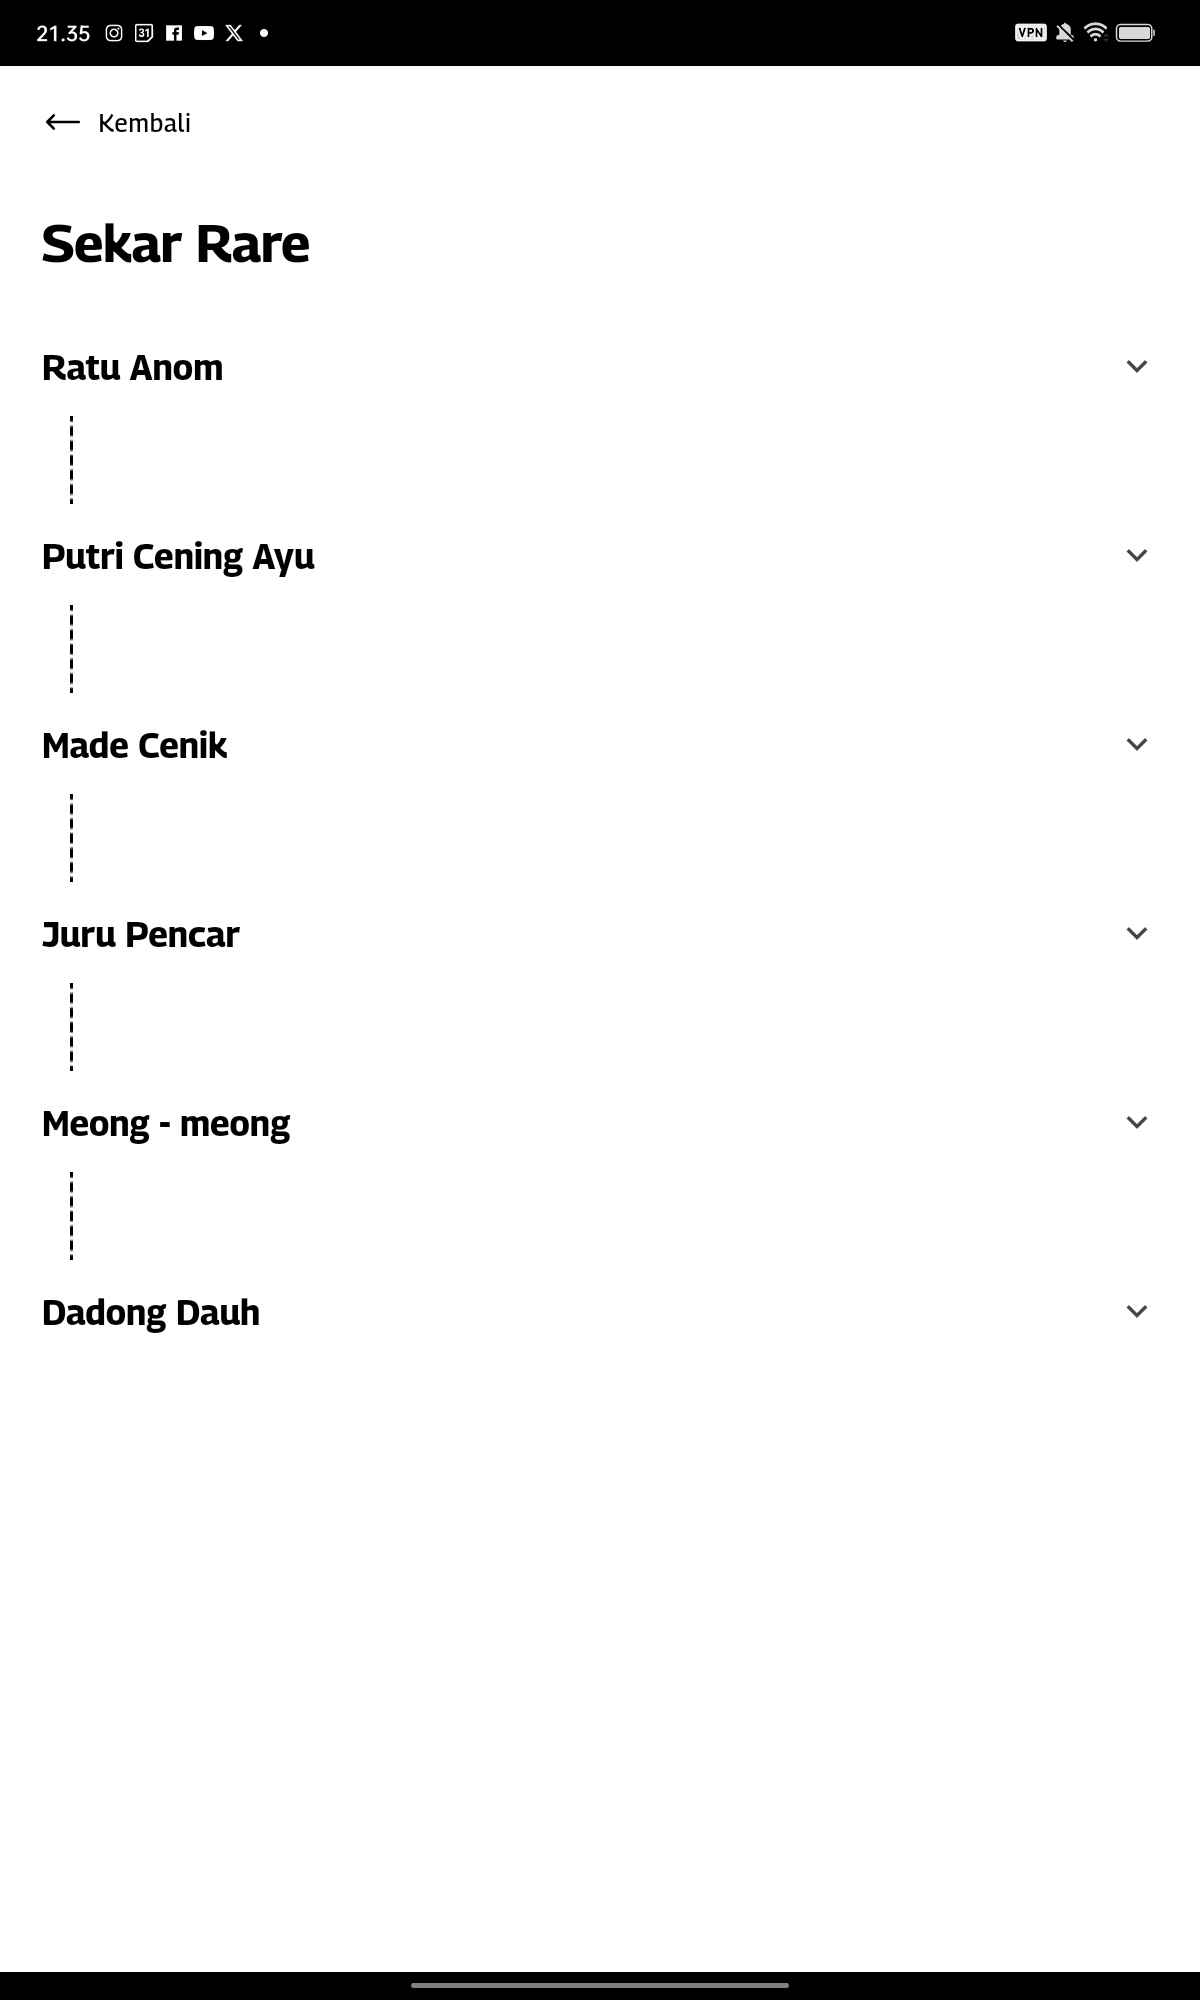
\includegraphics[width=0.3\textwidth]{assets/list-rare.jpg}
    \caption{List Sekar}
\end{figure}

\subsubsection{Pilih Sejarah Tembang}
Pilih Sejarah Tembang untuk melihat Penjelasan.

\begin{figure}[H]
    \centering
    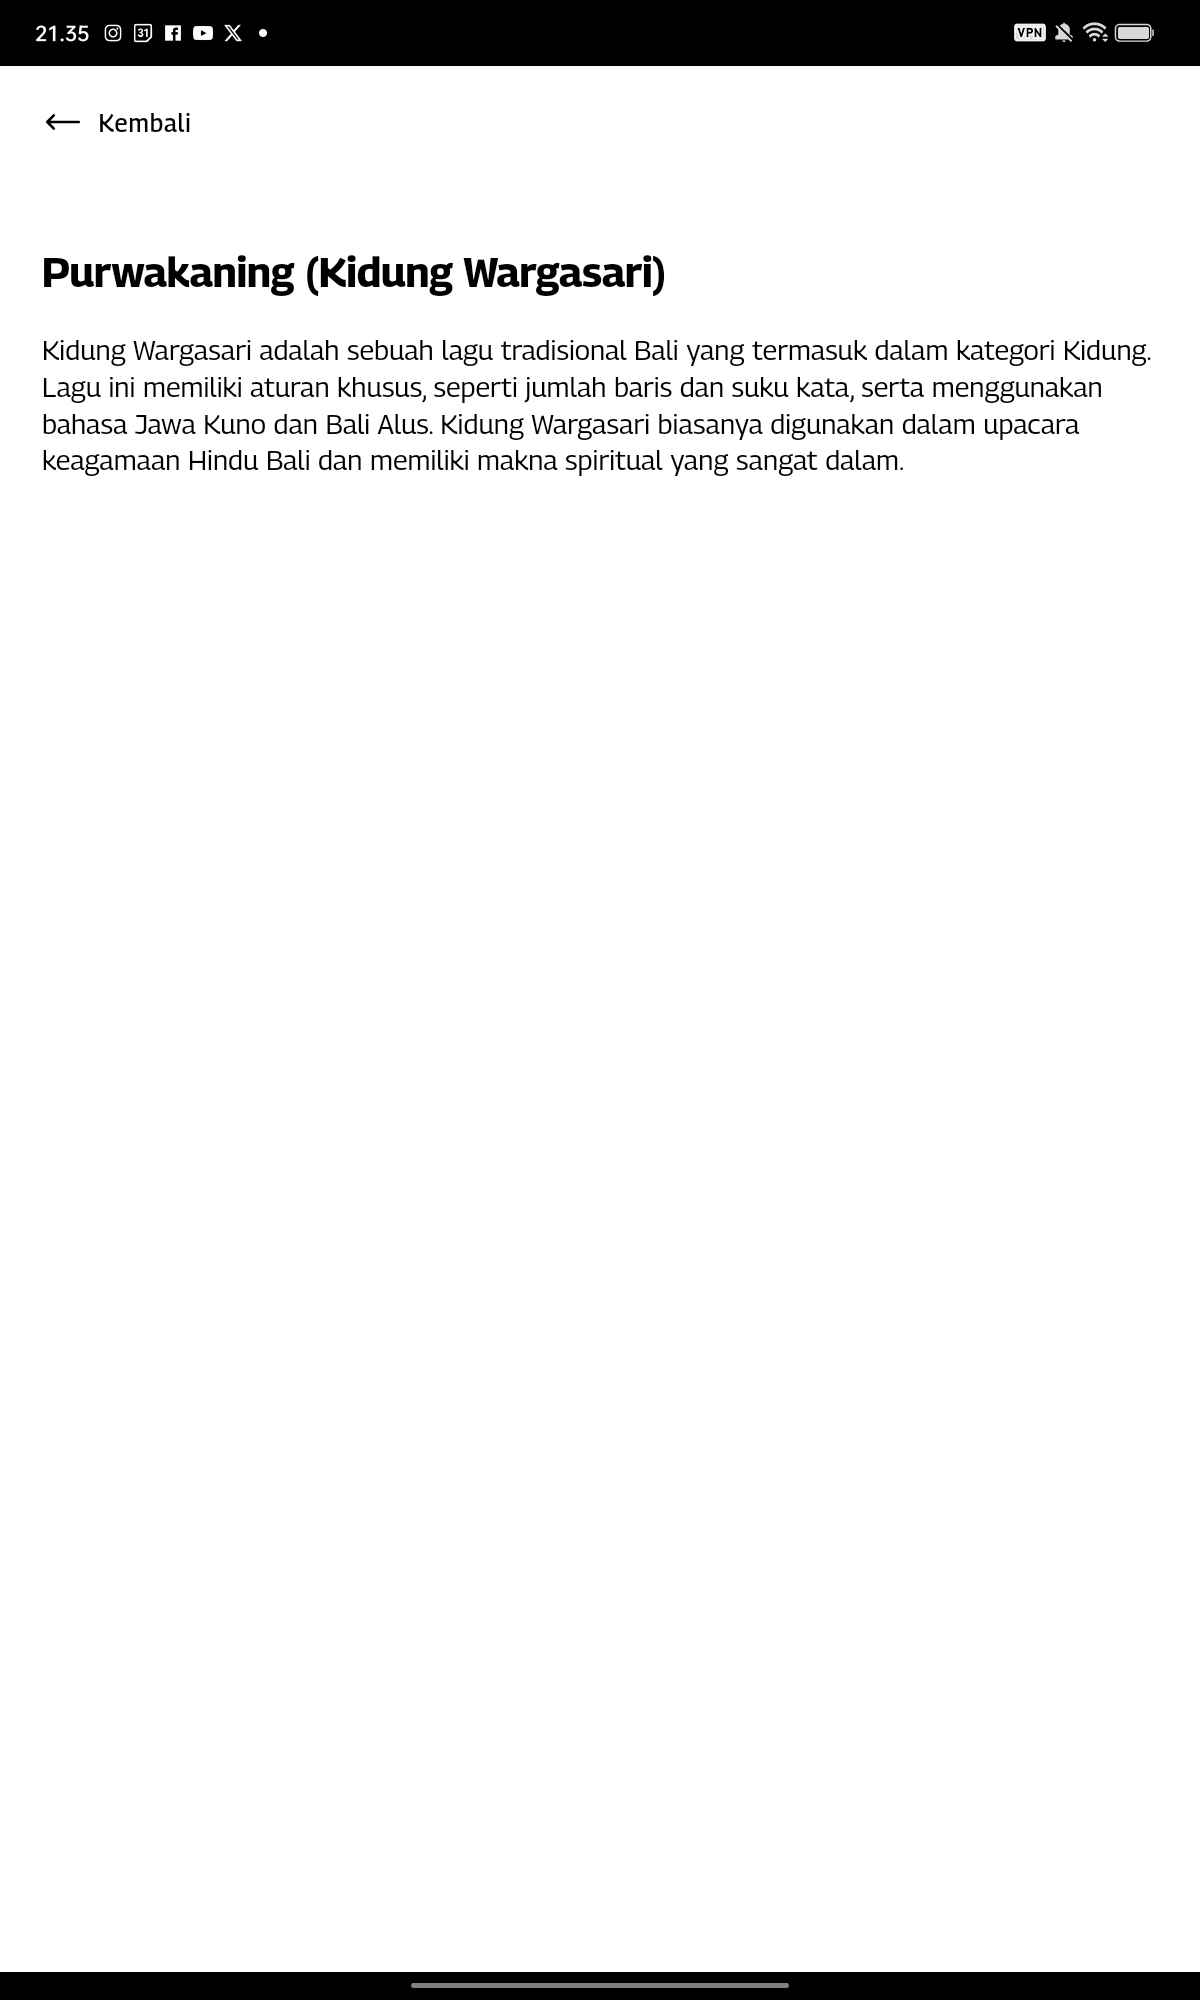
\includegraphics[width=0.3\textwidth]{assets/explanation.jpg}
    \caption{Login Page}
\end{figure}

\subsubsection{Pilih Lagu/Karaoke}
Pilih Karaoke untuk melihat lirik dan memutar lagu

\begin{figure}[H]
    \centering
    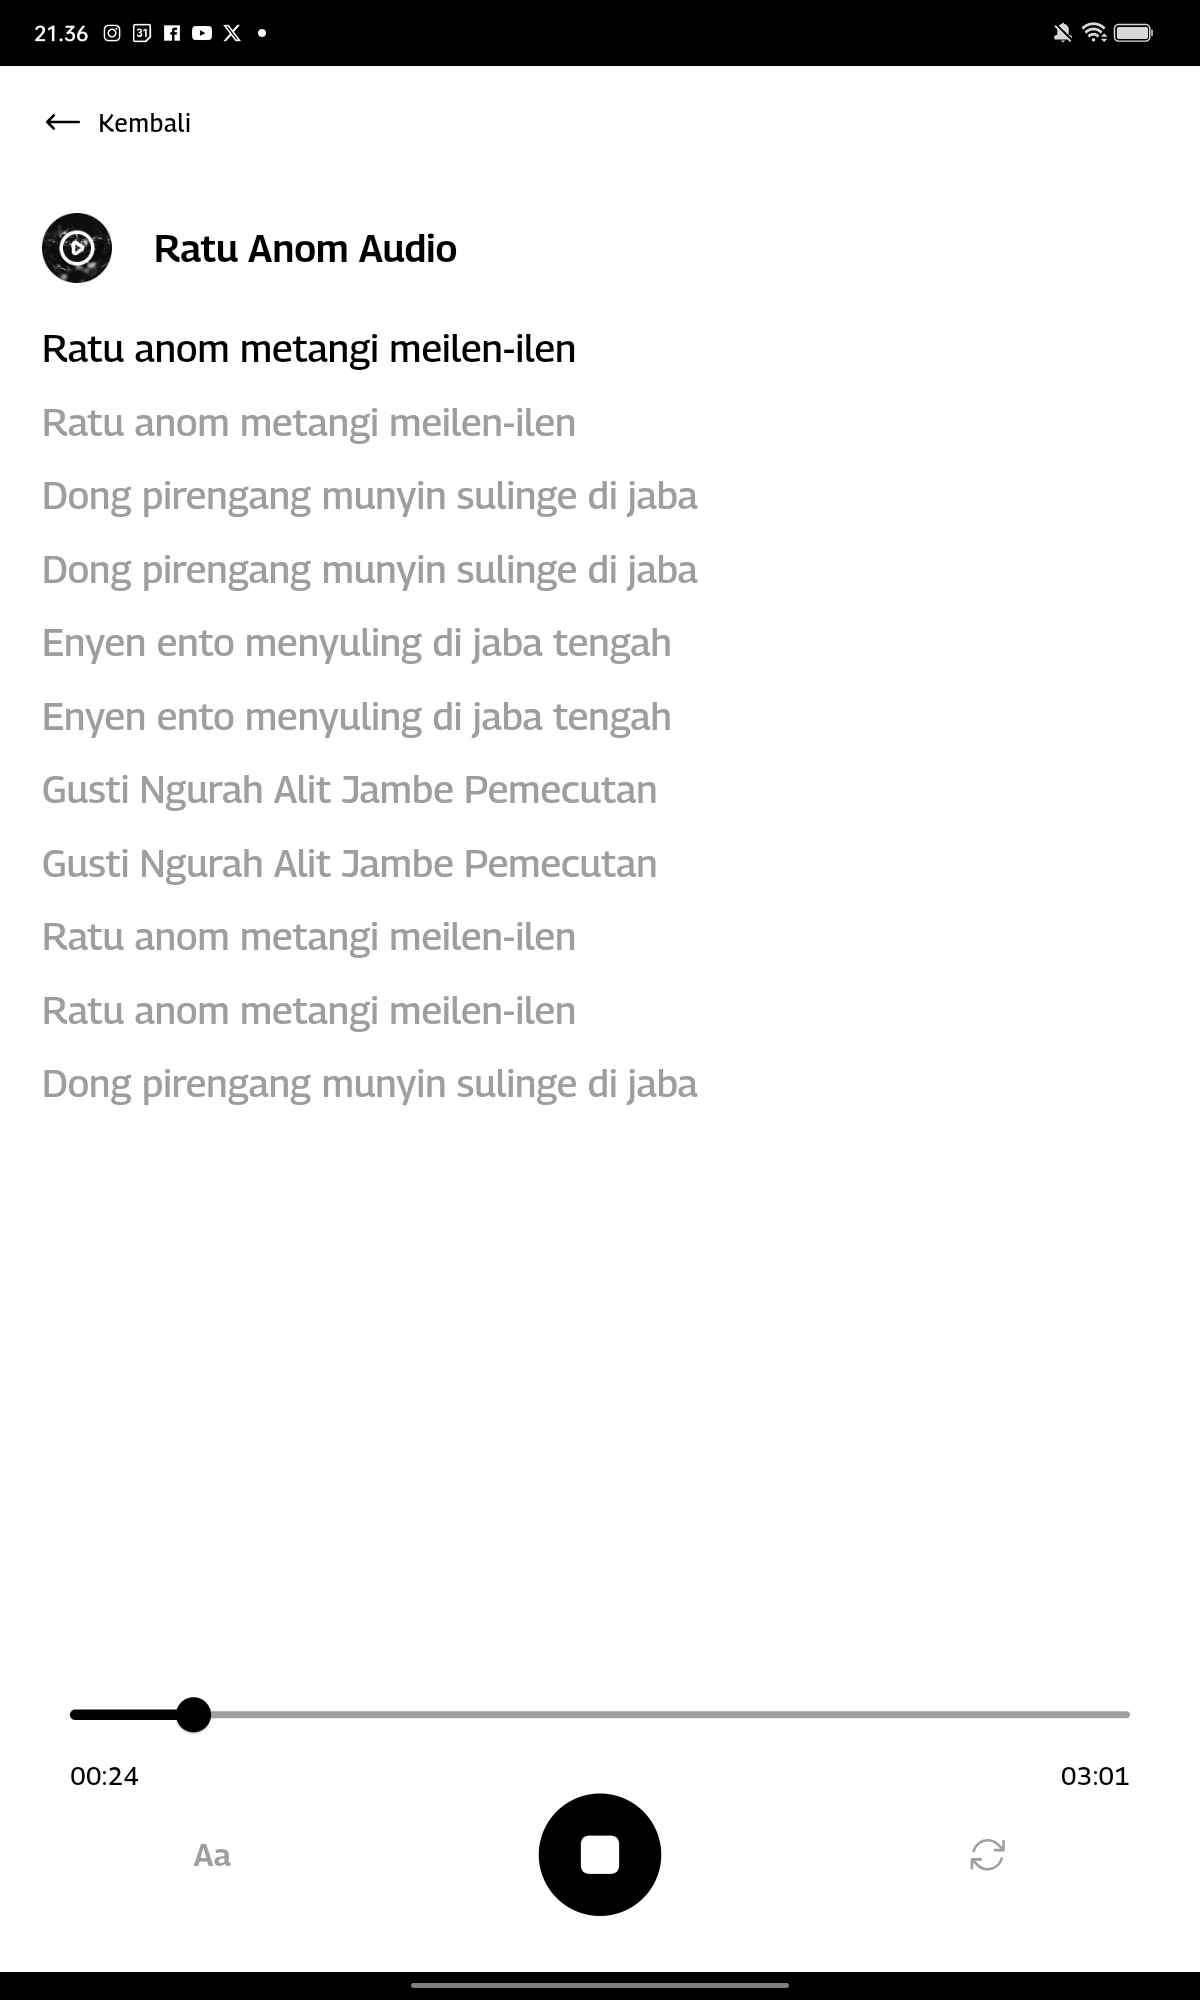
\includegraphics[width=0.3\textwidth]{assets/lyric.jpg}
    \caption{Login Page}
\end{figure}

\section{Manual Penggunaan Web Admin}

\subsection{Input Data}
Sistem Tembang Bali terdiri atas 2 komponen utama yaitu, \textit{server} dan \textit{client}.

\subsubsection{Buka Web}
Bukalah website webadmin tembang bali pada \href{https://tembang.fuwuna.tech/_}{Link Webadmin}
Akan muncul tampilan seperti dibawah ini.

\begin{figure}[H]
    \centering
    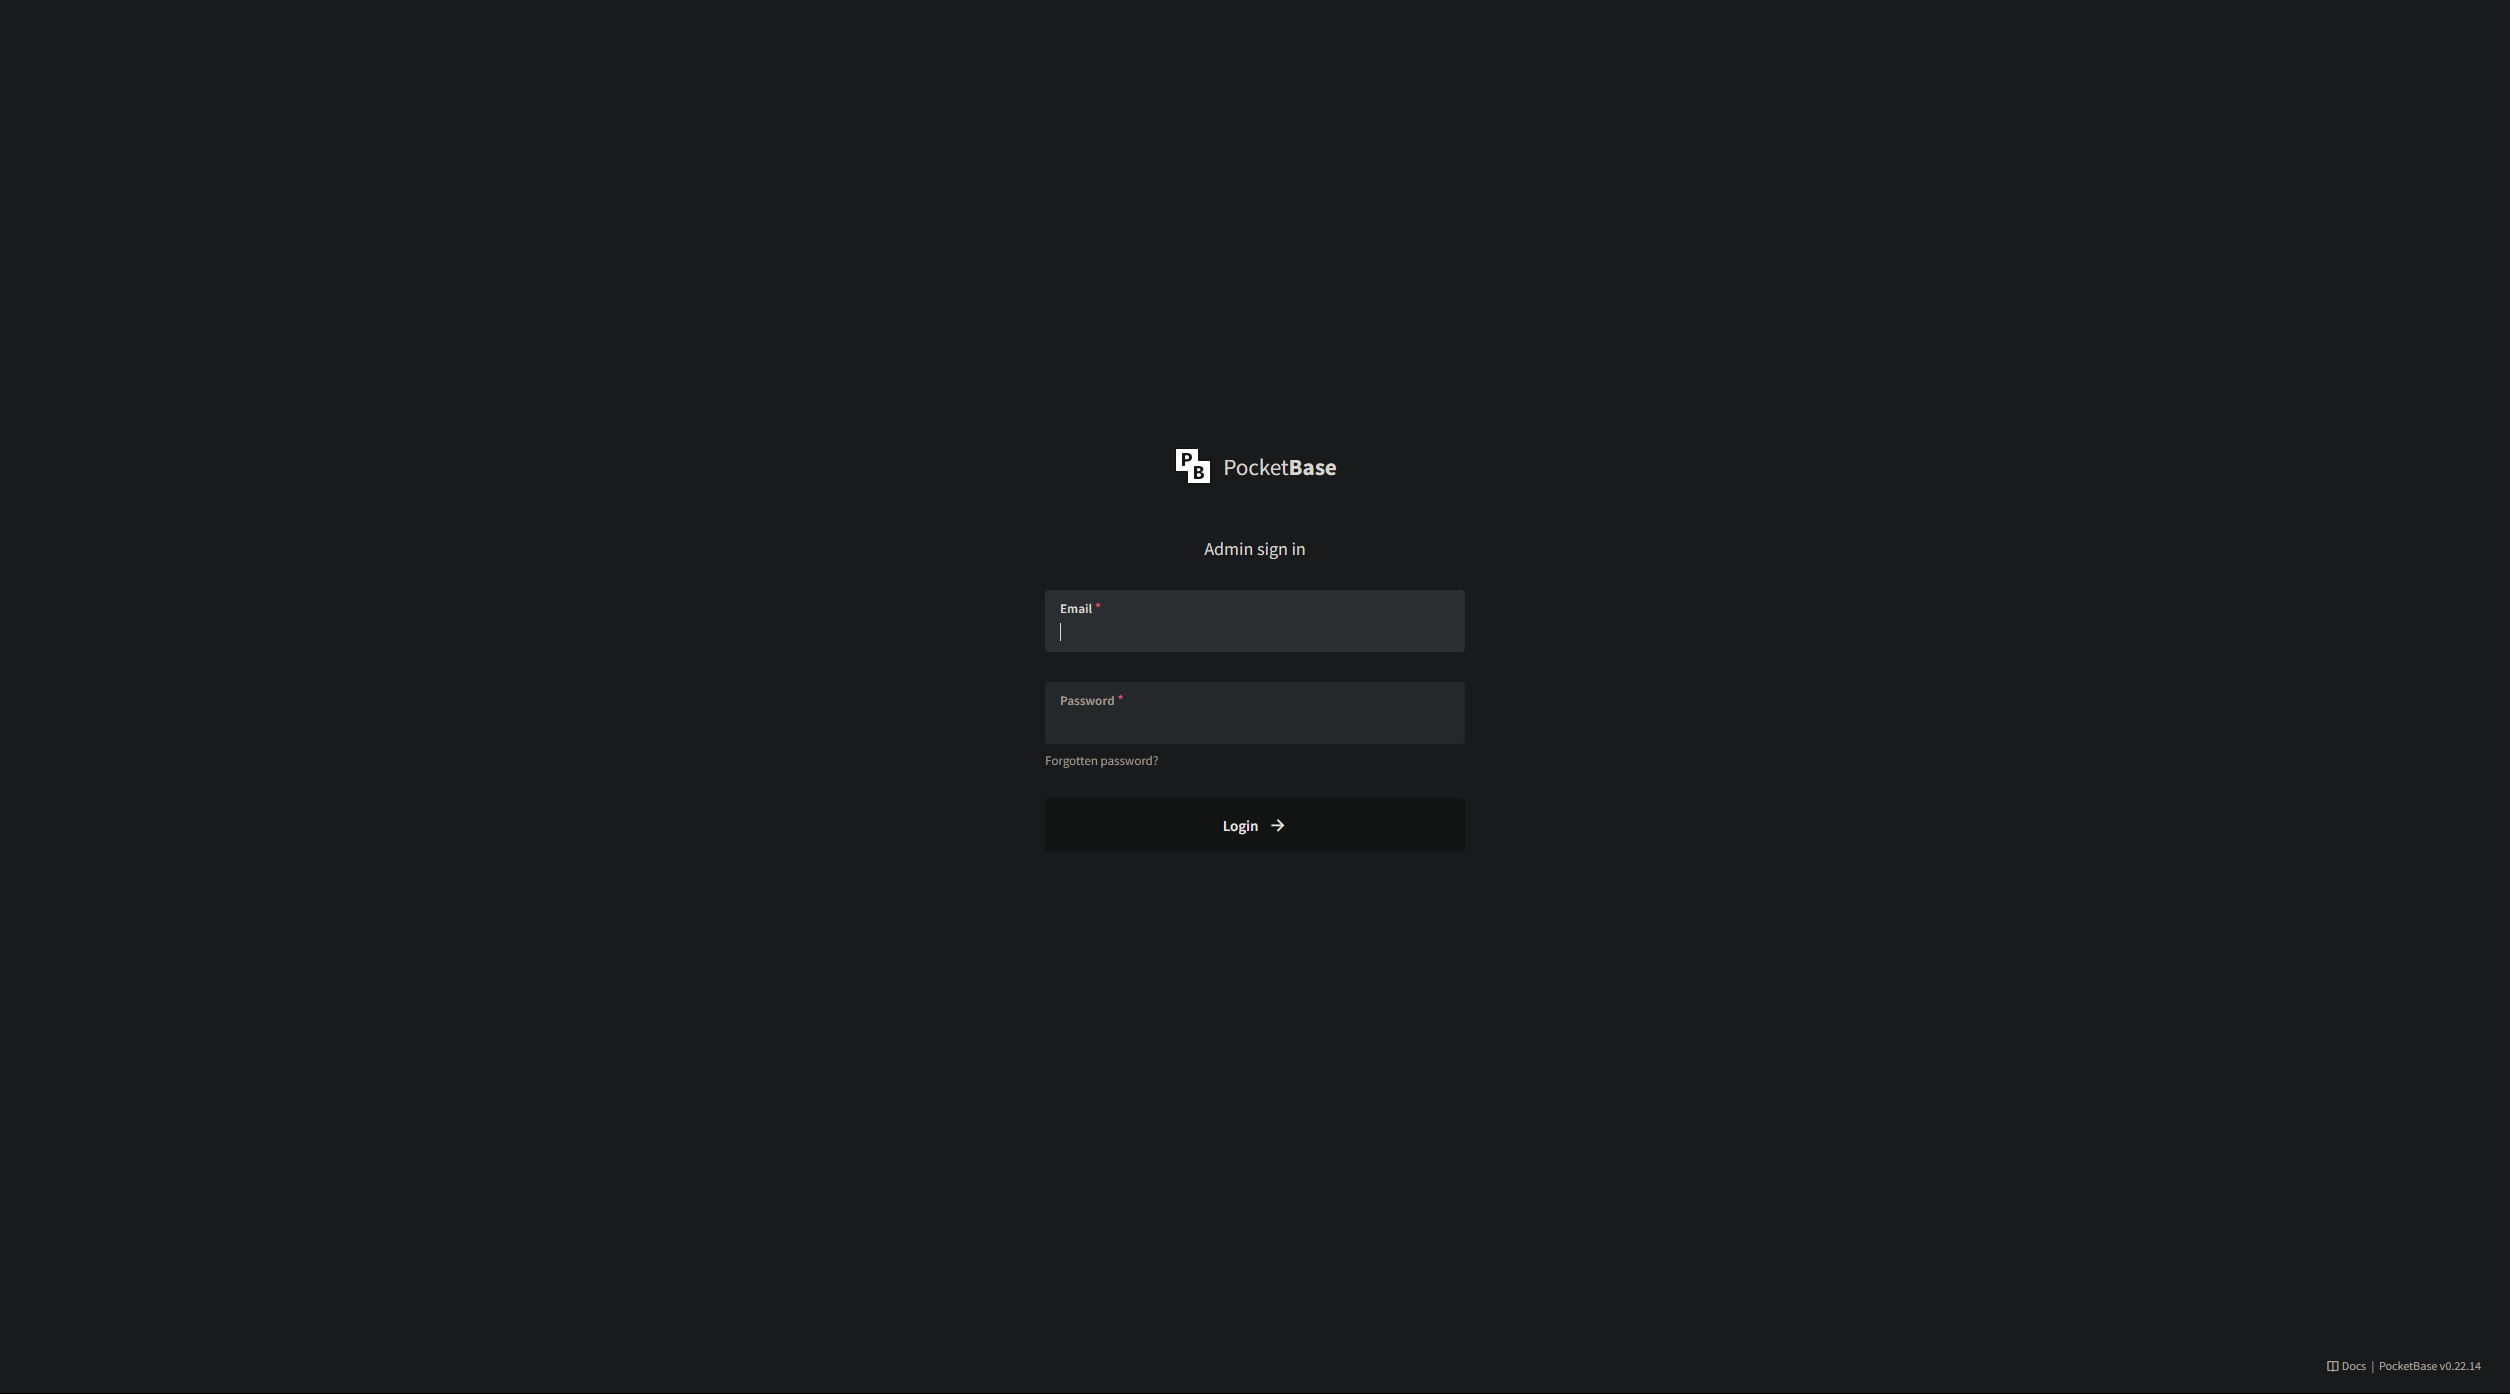
\includegraphics[width=0.8\textwidth]{assets/webview.png}
    \caption{Login Page}
\end{figure}

\subsubsection{Login ke Web}
Login ke web dengan akun email dan password yang sudah diberikan oleh admin tembang bali.
Setelah login akan muncul tampilan seperti dibawah ini.


\begin{figure}[H]
    \centering
    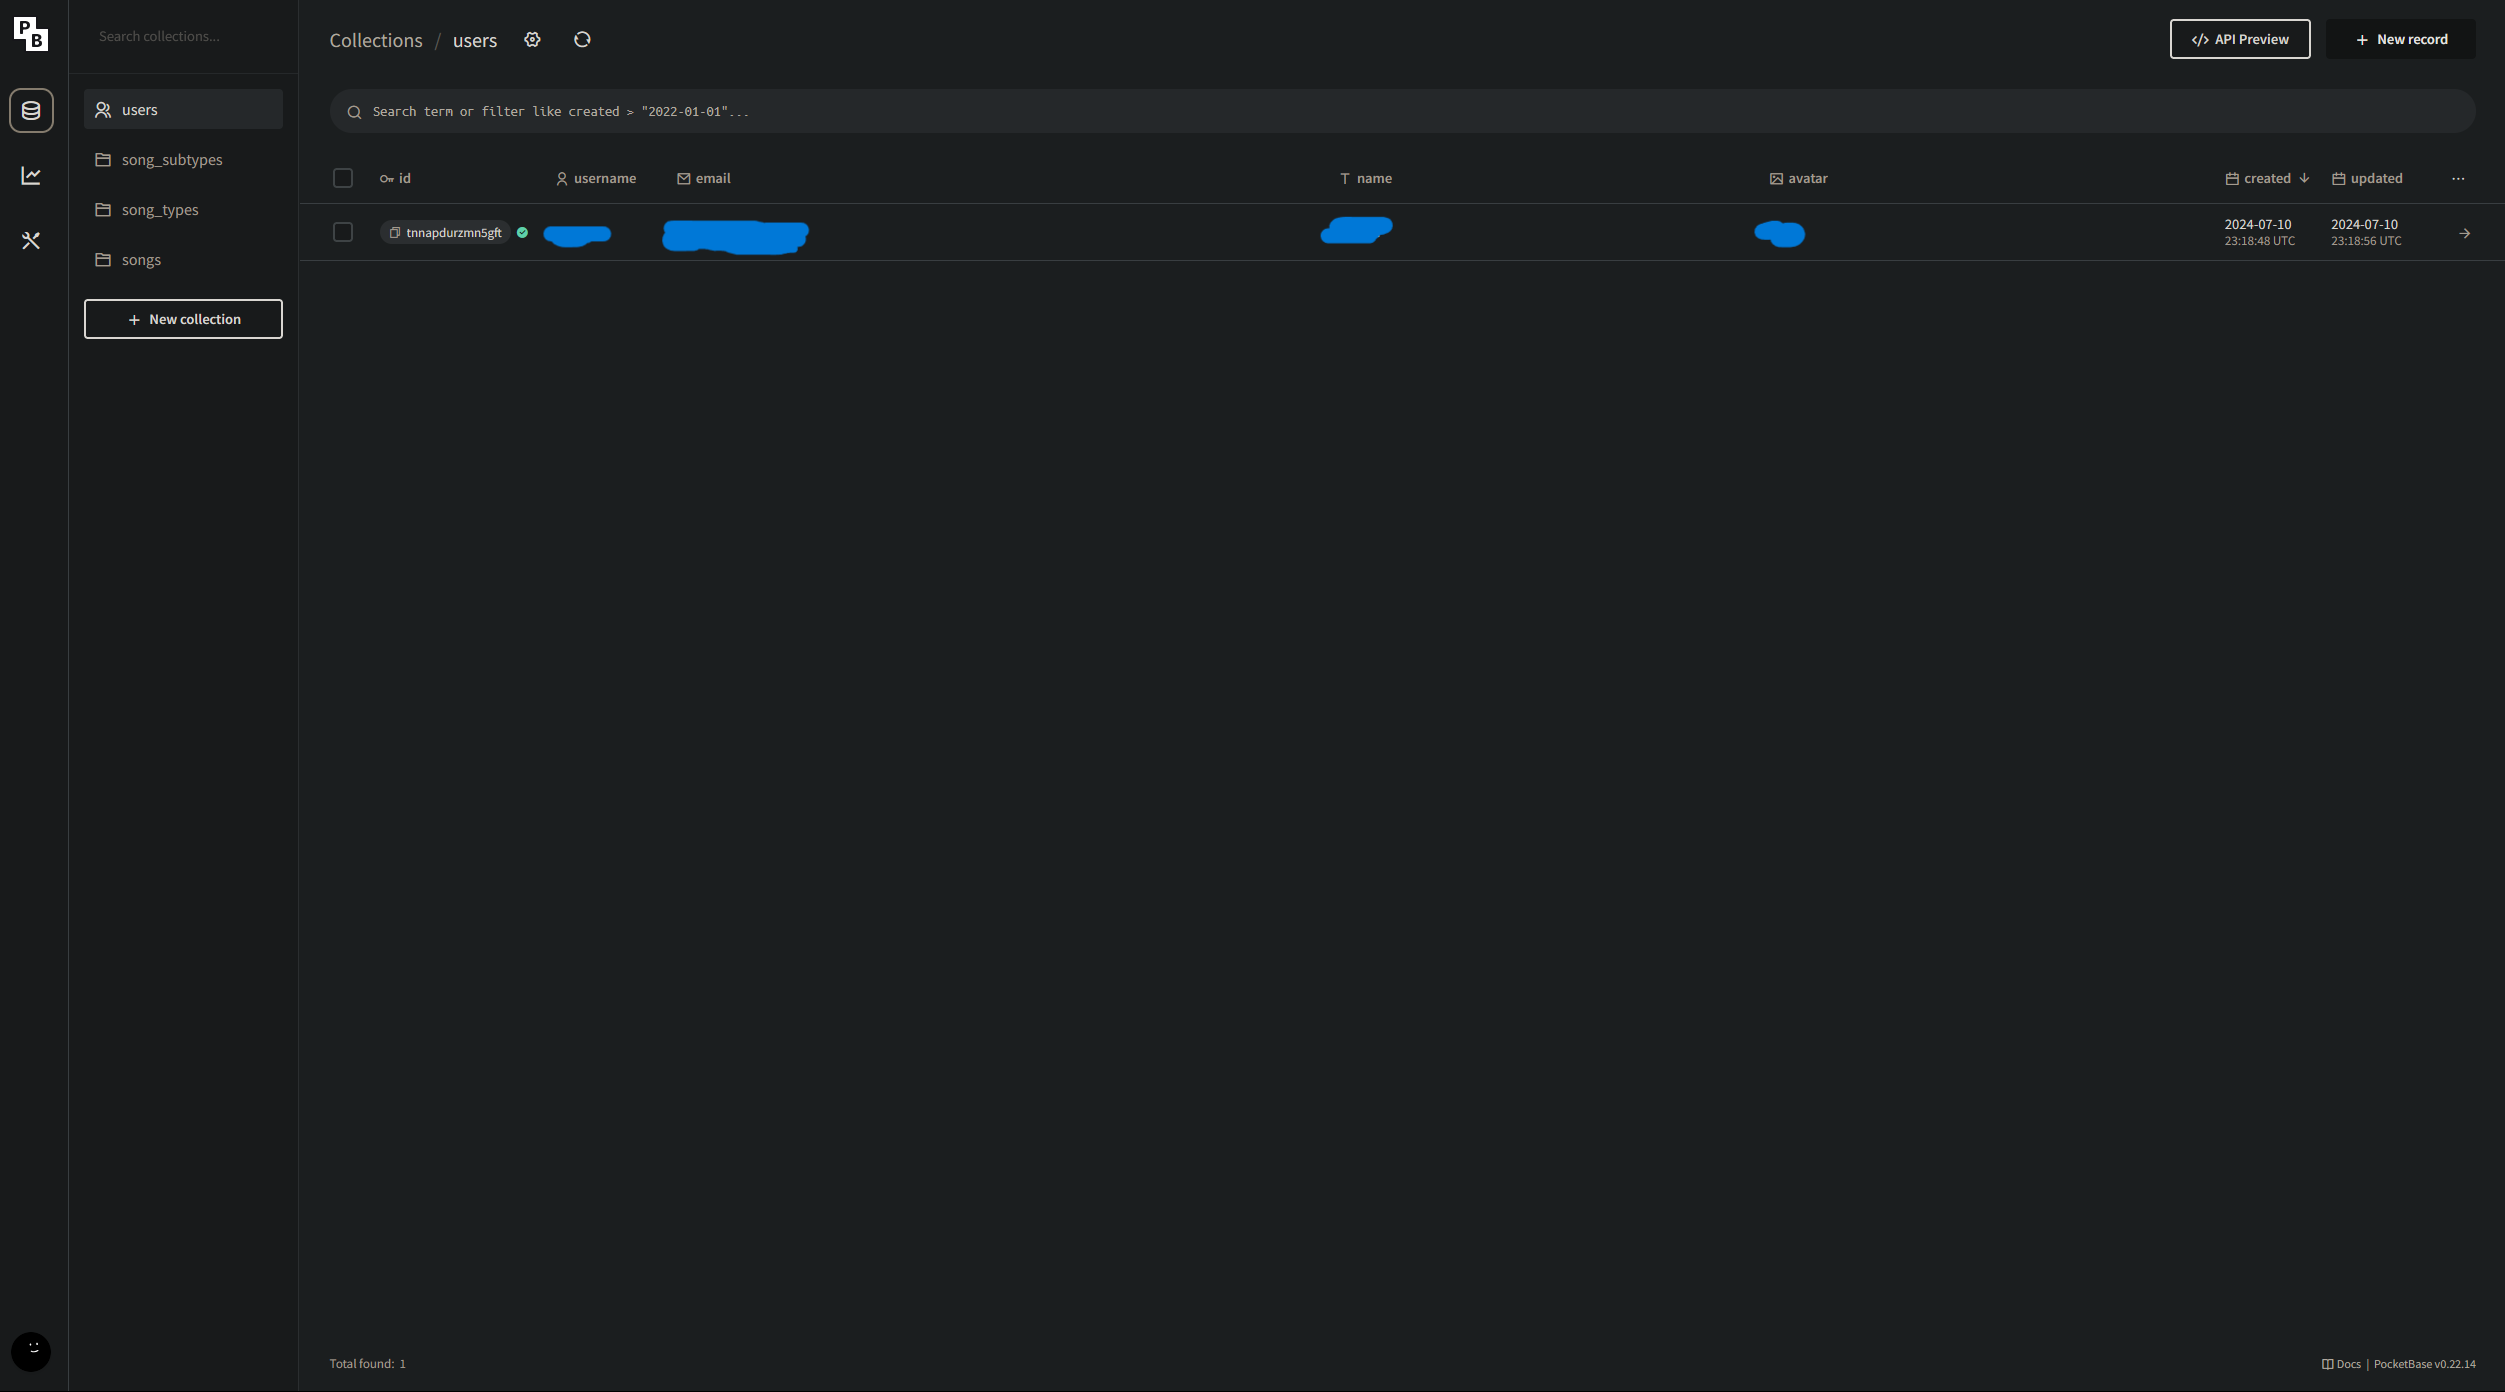
\includegraphics[width=0.8\textwidth]{assets/app.png}
    \caption{Tampilan Webadmin}
\end{figure}


\subsubsection{New Record}
Klik New Record pada pojok kanan atas untuk membuka form input

\begin{figure}[H]
    \centering
    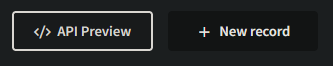
\includegraphics[width=0.8\textwidth]{assets/new-record.png}
    \caption{Tombol New Record}
\end{figure}

\subsubsection{Isi Form}
Isi semua data yang dibutuhkan kecuali id, pada form dengan data yang diinginkan kemudian klik tombol Create untuk menyimpan data

\begin{figure}[H]
    \centering
    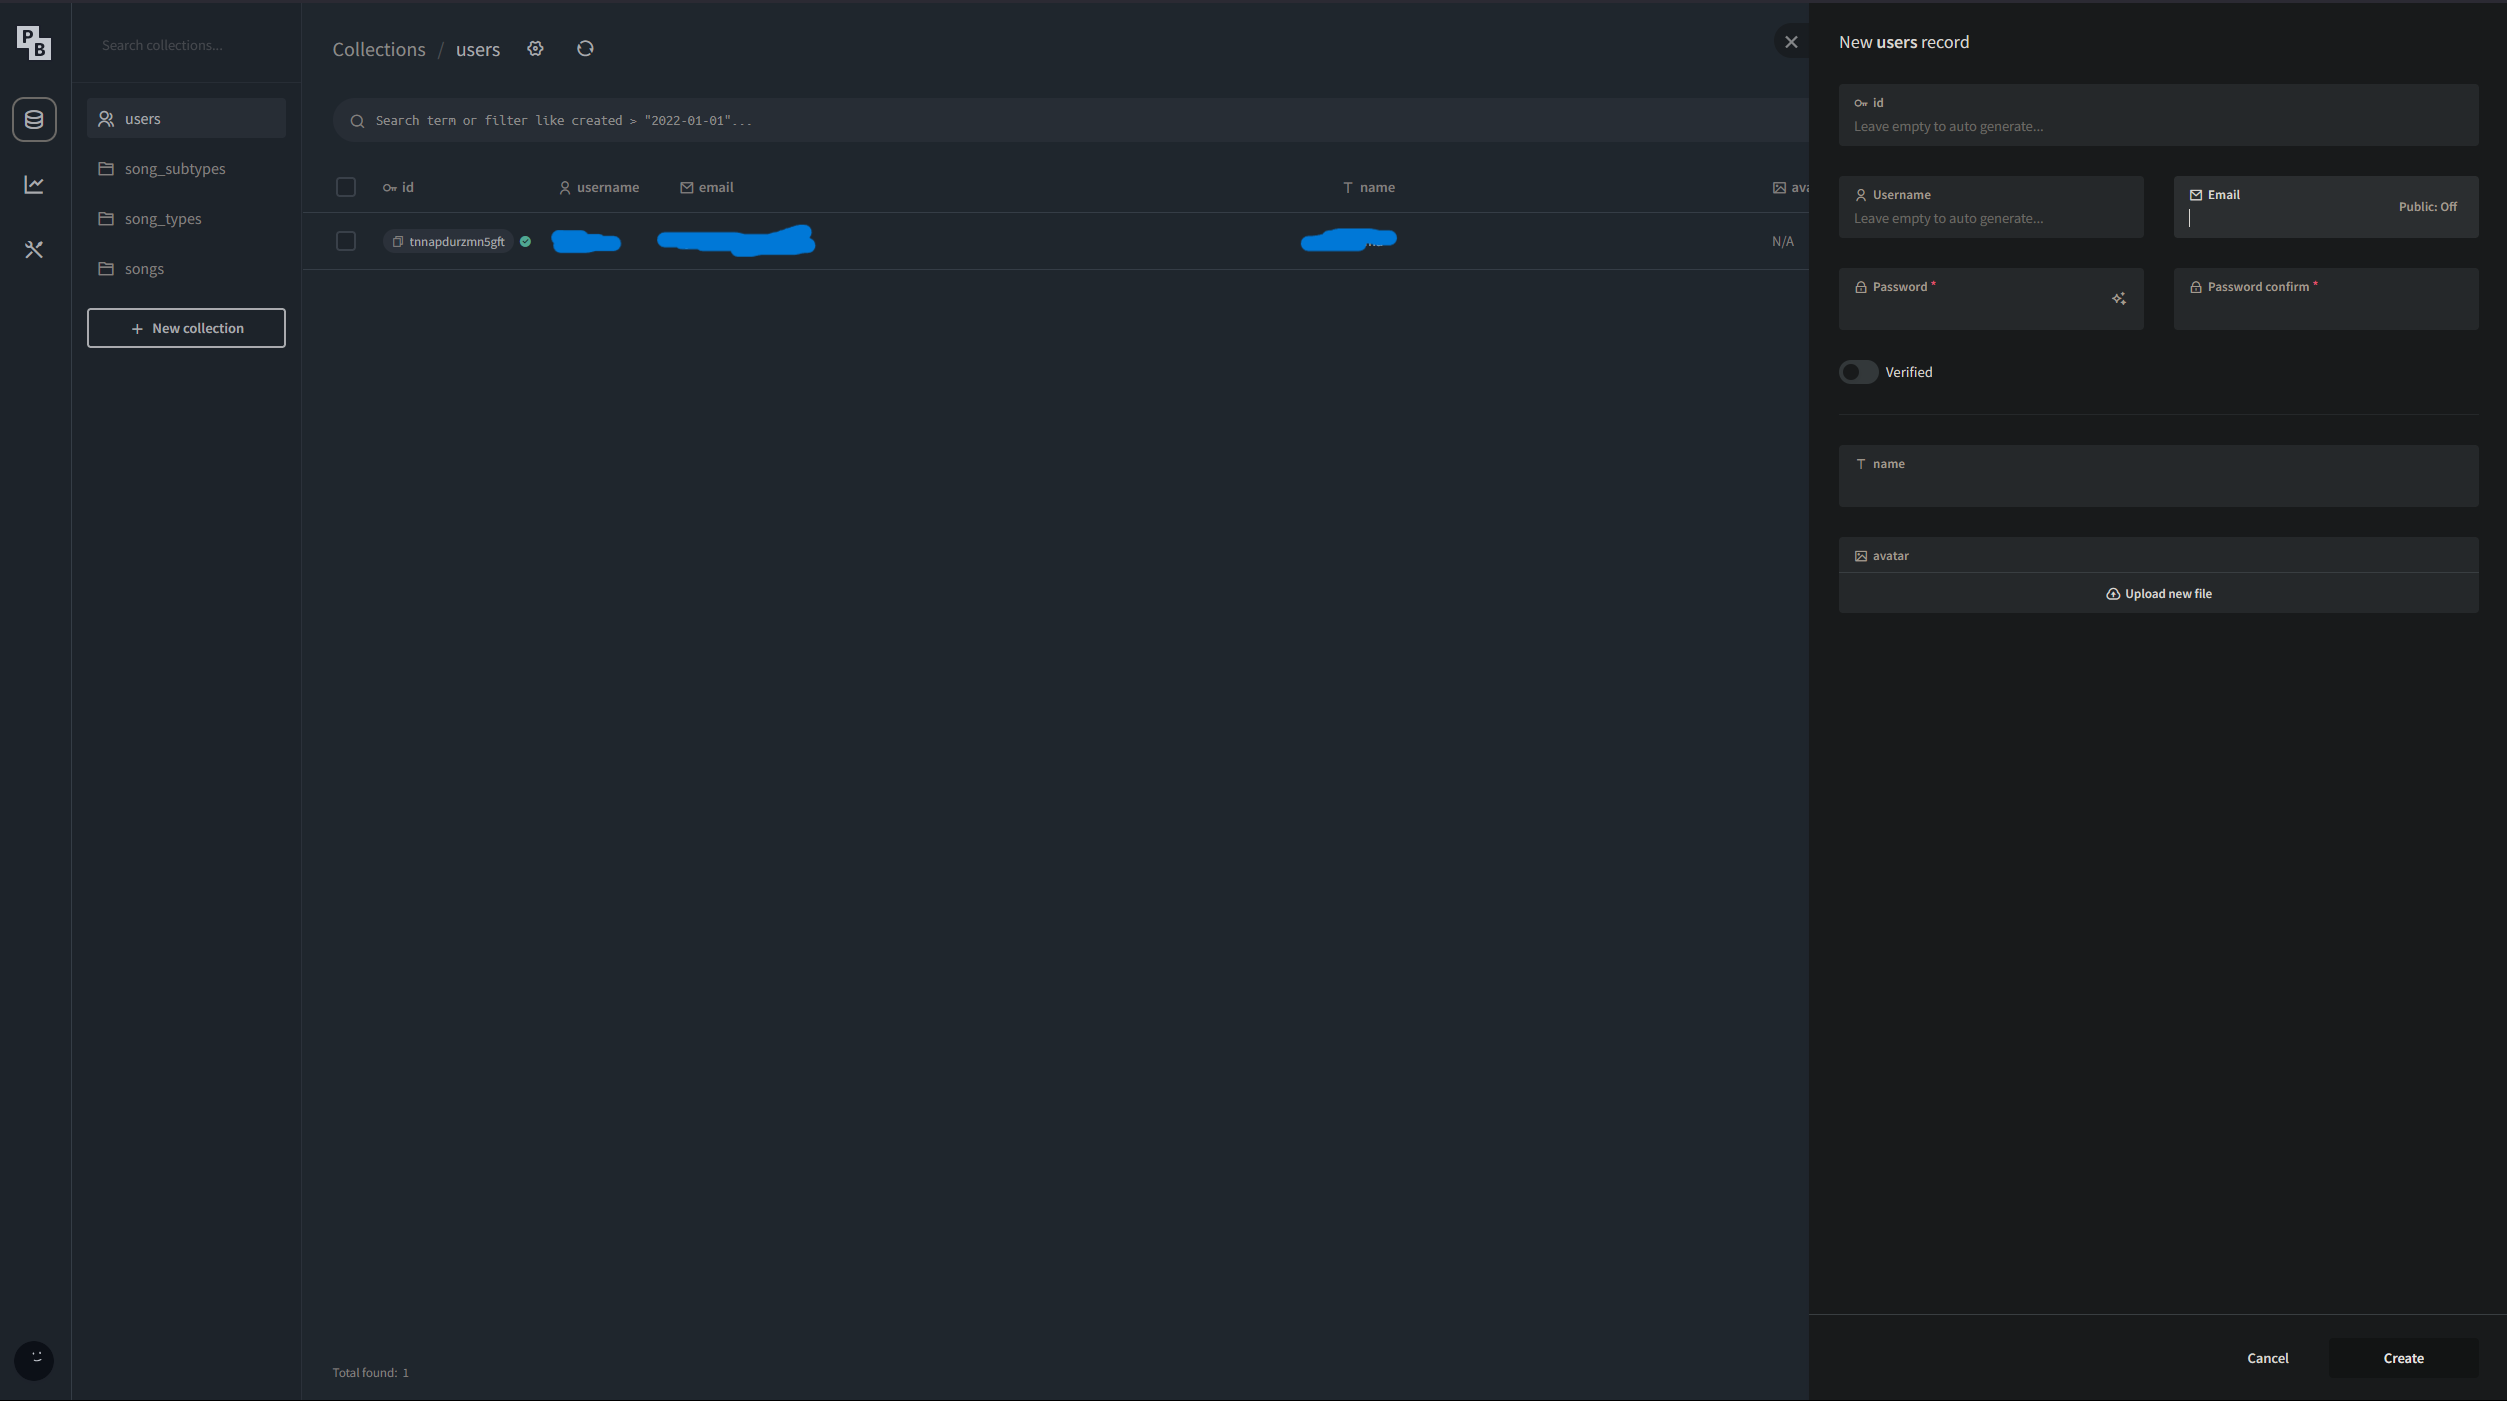
\includegraphics[width=0.8\textwidth]{assets/form.png}
    \caption{Form Input}
\end{figure}

\begin{figure}[H]
    \centering
    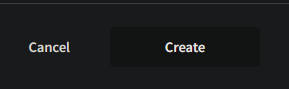
\includegraphics[width=0.8\textwidth]{assets/create.png}
    \caption{Form Input}
\end{figure}